\section{Fuge in g-moll, BWV 861, T.~24ff}

Fast hätten wir bei unseren Analysen im Unterricht diese Fuge ausgelassen, da sie -- wahrscheinlich spätestens seit den Analysen von Erwin Ratz -- als Paradebeispiel für die Form von Bach Fugen verwendet wurde.

\begin{quote}
"<Dem Schema am nächsten steht die \emph{g-moll Fuge} des ersten Bandes.">\autocite[80f]{ratz:formenlehre}
\end{quote}

Wir wollten aber durch eigene Analysen herausfinden, warum diese Fuge als Lehrbeispiel so gut geeignet ist.
Unsere Untersuchungen haben ergeben, dass dies wahrscheinlich deshalb so ist, weil die Durchführungen sehr regelmässig aufgebaut sind und einem klaren Tonartenplan folgen\footnote{1.~Durchführung in \emph{g-moll}, 2.~Dfg. in \emph{B-dur}, 3.~Dfg. in \emph{c-moll}, 4. und 5.~Dfg. wieder in \emph{g-moll}}.
Ausserdem geht die 2.~Durchführung noch einmal, fast wie in der Exposition, durch alle Stimmen; abgesehen davon, der vierte Themeneinsatz in T.~17 in der Tenorlage hier erneut als Basseinsatz erklingt.
Ein weiterer Punkt wäre, dass diese \emph{Fuga à 4 voci} erst relativ spät in der 2.~Durchführung ab Takt 15 tatsächlich vierstimmig wird und vorher maximal drei Stimmen erklingen, was vor allem in der Exposition einer vierstimmigen Fuge etwas überrascht.

Eher untypisch ist bei dieser Fuge hingegen, dass zwischen den Durchführungen keine regelmässigen Sequenzen komponiert sind, sondern nur Orgelpunkte, Kadenzmodelle und \emph{harmonische Sequenzen}.
Erst am Ende der Fuge zwischen den beiden letzten Durchführungen, beide in \emph{g-moll}, erklingt eine regelmässige Sequenz die mit drei Sequenzgliedern sogar relativ lang ist.
Die besondere Ausarbeitung Bachs der Dissonanzen und Verzierungen in dieser Romanesca-Sequenz\index{Romanesca} soll im Folgenden genauer untersucht werden.
In Abbildung~\ref{fig:bwv681-original} das Notenbeispiel dazu.

\begin{figure}[htbp]
	\centering
	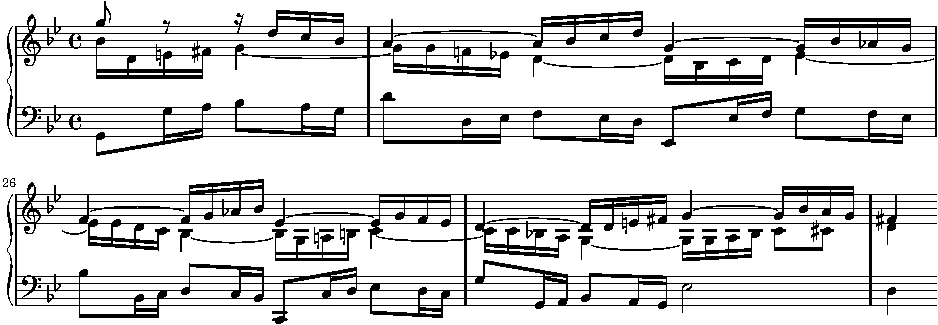
\includegraphics{lilypond/g-moll/render/original}
	\caption{Fuge in g-moll, BWV~861, T.~24ff}
	\label{fig:bwv681-original}
\end{figure}

Um einen Ausgangspunkt für weitere Analysen zu haben sei in Abbildung~\ref{fig:bwv681-romanesca-standard} die Standard Romanesca über Bachs Bass mit der üblichen 4--3 9--8 Bezifferung gegeben.

\begin{figure}[htbp]
	\centering
	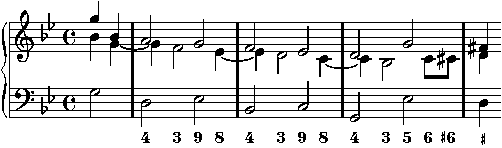
\includegraphics{lilypond/g-moll/render/romanesca-standard}
	\caption{Typische Romanesca mit 3-2-consecutive in den Oberstimmen}
	\label{fig:bwv681-romanesca-standard}
\end{figure}


\subsection{Ausarbeitung der Synkopenkette in den Oberstimmen}

In der Sequenz von Bach ist diese Romanesca allerdings nicht in dieser Schlichtheit komponiert.
Stattdessen entsteht bei ihm durch die verzierten Oberstimmen und den figurierten Bass eine andere Ausarbeitung der zu Grunde liegenden Romanesca-Sequenz, die dadurch einen völlig anderen Charakter bekommt.
Die harmonische Reduktion mit Generalbassbezifferung ist in Abbildung~\ref{fig:bwv681-vorhalte} gesetzt.

\begin{figure}[htbp]
	\centering
	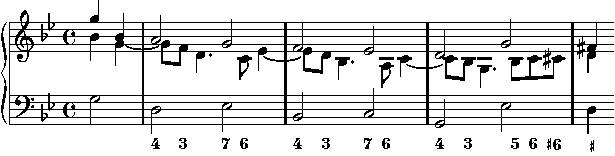
\includegraphics{lilypond/g-moll/render/romanesca-vorhalte}
	\caption{Bachs Harmonisierung der Romanesca-Sequenz in der Fuge in g-moll, BWV~861, T.~24ff}
	\label{fig:bwv681-vorhalte}
\end{figure}

Es ist schwer zu sagen, ob diese besondere Bezifferung der Romanesca-Sequenz mit 4--3 7--6 die kompositorische Idee war, oder das Resultat der Verzierungen in den beiden Oberstimmen die hier im Weiteren besprochen werden.
Bemerkenswert ist aber auf jeden Fall, dass durch eine so einfache Veränderung im Generalbass und einer Unterbrechung der regulären 3-2-consecutive eine recht besondere Sequenz resultiert die alleine dadurch dem Bachstil womöglich schon etwas näher kommt.

Der nächste Schritt um der originalen Komposition Bachs näher zu kommen wäre die in Abbildung~\ref{fig:bwv681-vorhalte} entstandenen \emph{patiens}-Stimme mit Verzierungen zu umspielen.
Hierfür füllt Bach alle in Achtelnoten aufeinander folgenden Terzen mit einem Durchgang auf.
Ausserdem erweitert er die so entstandene kleine Sechzehntelfigur durch ein weiteres, vorangestelltes Sechzehntel, sodass daraus eine Tonleiter von drei Tönen entsteht die auftaktig zum nächsten Ton auf einer schweren Zählzeit hinführt.
In Abbildung~\ref{fig:bwv681-patiens-verziert} kann Bachs Ausarbeitung gesehen werden; hier nach wie vor mit der vereinfachten \emph{parte agens}-Stimme.

\begin{figure}[htbp]
	\centering
	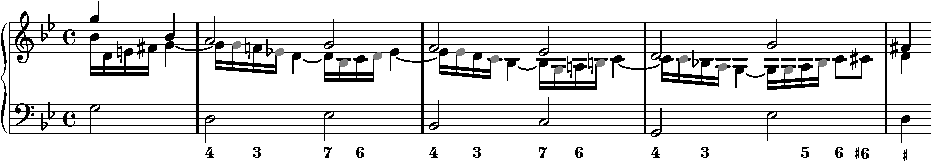
\includegraphics{lilypond/g-moll/render/romanesca-patiens-verziert}
	\caption{Bachs Figurationen der \emph{parte patiens}-Stimme in der Fuge in g-moll, BWV~861, T.~24ff}
	\label{fig:bwv681-patiens-verziert}
\end{figure}

Auf den leichten Sechzehntel-Zählzeiten erklingen also verschiedene Dissonanzen, die aber alle im Sinne der Figurenlehre von Heinrich Schütz\autocite{bernhard:kompositionslehre} erklärt werden können.

\begin{itemize}
\item
	In Takt 25 kann das erste \emph{g\textsuperscript{1}} (2.~Sechzehntel) als \emph{Multiplicatio}\autocite[203f]{bartel:figurenlehre}\autocite[75]{bernhard:kompositionslehre} verstanden werden.
	Es ist also eine Verlängerung der dissonante Quarte.
\item
	Das \emph{es\textsuperscript{1}} (4.~Sechzehntel) ist wie oben bereits beschrieben ein regulärer Durchgang (vgl.\emph{Transitus} bei Bartel\autocite[260ff]{bartel:figurenlehre} oder Bernhard\autocite[64f]{bernhard:kompositionslehre}).
\item
	Das \emph{b} (10.~Sechzehntel) ist eine Figur mit besonderer Wirkung.
	Mit dieser \emph{Subsumtio} wird die Auflösung der Dissonanz (hier als Septime) erreicht in dem die Note unter der auflösenden Note angesprungen wird und diese schliesslich durch einen Aufwärtsschritt erreicht wird (vgl.\emph{Subsumtio} bei Bartel\autocite[242ff]{bartel:figurenlehre} oder Bernhard\autocite[148f]{bernhard:kompositionslehre}).
\item
	Das \emph{d\textsuperscript{1}} (12.~Sechzehntel) kann hier ebenfalls als \emph{Transitus} erklärt werden, hier aber im Gegensatz zu vorher aufwärts.
\end{itemize}

Entsprechend verhält es sich mit den dissonanten Noten auch in den weiteren Takten und Sequenzgliedern.
Bemerkenswert ist ausserdem, dass diese Sechzehntelfigurationen abwechselnd aufwärts und abwärts gesetzt sind.

Das einzige was jetzt noch fehlt um von der 3-2-consecutive auf Bachs Satz zukommen ist die Figuration der Oberstimme. In Abbildung~\ref{fig:bwv681-agens-verziert} nun die vollständig ausgearbeitet Synkopenkette.

\begin{figure}[htbp]
	\centering
	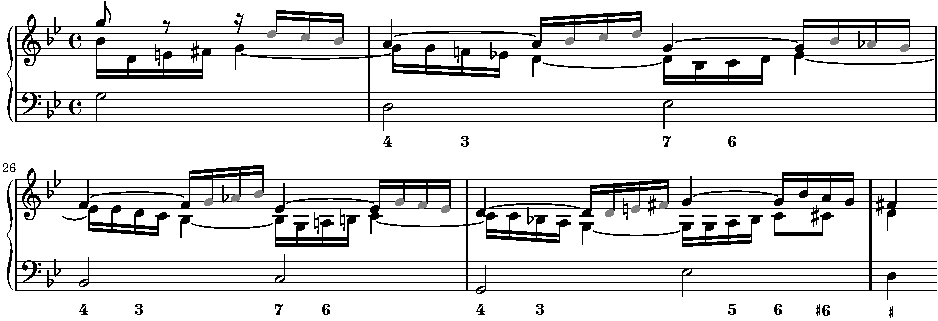
\includegraphics{lilypond/g-moll/render/romanesca-agens-verziert}
	\caption{Bachs Figuration der \emph{agens}-Stimme in der Synkopenkette der Romanesca-Sequenz der Fuge in g-moll, BWV~861, T.~24ff}
	\label{fig:bwv681-agens-verziert}
\end{figure}

Diese Stimme ist in der Figuration etwas freier als die \emph{patiens}-Stimme, da die keine Dissonanzen vorbereiten und auflösen muss.
Dennoch findet Bach auch hier eine Figuration die sich Rhythmisch parallel zu der \emph{patiens}-Stimme verhält; also einmal der Auftakt der drei Sechzehntel abwärts und einmal aufwärts.
Daraus resultiert nun ein faszinierendes Phänomen.
Liest man die Figuration der Oberstimme auf dem 4.~Viertel in Takt 24 zusammengefasst mit der Unterstimme auf dem 1.~Viertal in Takt 25, so ergibt sich daraus eine komplette diatonische Tonleiter abwärts (in phrygisch).

Auch in in den darauf folgenden zwei Figurationen als eine zusammengefasst wird man feststellen können, dass dort sowohl in der Oberstimme wie auch in der Unterstimme die exakt gleichen Töne \emph{b-c-d} erklingen, aber einmal als \emph{6-7-8} in \emph{d-moll} und einmal als \emph{5-6-7} zu \emph{Es-dur}, bzw. hier eher \emph{7-1-2-3} in \emph{c-moll}, da in dieser Romanesca wie oben Besprochen in der ersten Harmonie eines Sequenzgliedes nicht in den Grundakkord aufgelöst wird, sondern in einen Sextakkord.

Interessant ist auch, wie sich diese beide Besonderheiten mit der Tonleiter und den gleichen Tönen über die Grenzen der Sequenzgleider erstreckt.
In der Romanesca ist ein Sequenzglied ein Bass der eine Quarte fällt; das nächste Sequenzglied wird dann eine Terz versetzt.

% TODO: Der Bass der eine Quarte fällt und eine Sekunde steigt?


Lorem ipsum dolor sit amet, consectetur adipisicing elit, sed do eiusmod tempor incididunt ut labore et dolore magna aliqua. Ut enim ad minim veniam, quis nostrud exercitation ullamco laboris nisi ut aliquip ex ea commodo consequat. Duis aute irure dolor in reprehenderit in voluptate velit esse cillum dolore eu fugiat nulla pariatur. Excepteur sint occaecat cupidatat non proident, sunt in culpa qui officia deserunt mollit anim id est laborum.
